% This must be in the first 5 lines to tell arXiv to use pdfLaTeX, which is strongly recommended.
\pdfoutput=1
% In particular, the hyperref package requires pdfLaTeX in order to break URLs across lines.

\documentclass[11pt]{article}

% Change "review" to "final" to generate the final (sometimes called camera-ready) version.
% Change to "preprint" to generate a non-anonymous version with page numbers.
\usepackage[preprint]{acl}

% Standard package includes
\usepackage{times}
\usepackage{latexsym}

\usepackage{amsmath}
\usepackage{amsfonts}

% For proper rendering and hyphenation of words containing Latin characters (including in bib files)
\usepackage[T1]{fontenc}
% For Vietnamese characters
% \usepackage[T5]{fontenc}
% See https://www.latex-project.org/help/documentation/encguide.pdf for other character sets

% This assumes your files are encoded as UTF8
\usepackage[utf8]{inputenc}

% This is not strictly necessary, and may be commented out,
% but it will improve the layout of the manuscript,
% and will typically save some space.
\usepackage{microtype}

% This is also not strictly necessary, and may be commented out.
% However, it will improve the aesthetics of text in
% the typewriter font.
\usepackage{inconsolata}

%Including images in your LaTeX document requires adding
%additional package(s)
\usepackage{graphicx}

\newtheorem{hyp}{Hypothesis}

% If the title and author information does not fit in the area allocated, uncomment the following
%
%\setlength\titlebox{<dim>}
%
% and set <dim> to something 5cm or larger.

\title{Quantifying image realism via language model
reasoning}

% Author information can be set in various styles:
% For several authors from the same institution:
% \author{Author 1 \and ... \and Author n \\
%         Address line \\ ... \\ Address line}
% if the names do not fit well on one line use
%         Author 1 \\ {\bf Author 2} \\ ... \\ {\bf Author n} \\
% For authors from different institutions:
% \author{Author 1 \\ Address line \\  ... \\ Address line
%         \And  ... \And
%         Author n \\ Address line \\ ... \\ Address line}
% To start a separate ``row'' of authors use \AND, as in
% \author{Author 1 \\ Address line \\  ... \\ Address line
%         \AND
%         Author 2 \\ Address line \\ ... \\ Address line \And
%         Author 3 \\ Address line \\ ... \\ Address line}

\author{Kseniia Petrushina \\
  MIPT \\
  Skoltech \\
  \texttt{petrushina.ke@phystech.edu} \\}

%\author{
%  \textbf{First Author\textsuperscript{1}},
%  \textbf{Second Author\textsuperscript{1,2}},
%  \textbf{Third T. Author\textsuperscript{1}},
%  \textbf{Fourth Author\textsuperscript{1}},
%\\
%  \textbf{Fifth Author\textsuperscript{1,2}},
%  \textbf{Sixth Author\textsuperscript{1}},
%  \textbf{Seventh Author\textsuperscript{1}},
%  \textbf{Eighth Author \textsuperscript{1,2,3,4}},
%\\
%  \textbf{Ninth Author\textsuperscript{1}},
%  \textbf{Tenth Author\textsuperscript{1}},
%  \textbf{Eleventh E. Author\textsuperscript{1,2,3,4,5}},
%  \textbf{Twelfth Author\textsuperscript{1}},
%\\
%  \textbf{Thirteenth Author\textsuperscript{3}},
%  \textbf{Fourteenth F. Author\textsuperscript{2,4}},
%  \textbf{Fifteenth Author\textsuperscript{1}},
%  \textbf{Sixteenth Author\textsuperscript{1}},
%\\
%  \textbf{Seventeenth S. Author\textsuperscript{4,5}},
%  \textbf{Eighteenth Author\textsuperscript{3,4}},
%  \textbf{Nineteenth N. Author\textsuperscript{2,5}},
%  \textbf{Twentieth Author\textsuperscript{1}}
%\\
%\\
%  \textsuperscript{1}Affiliation 1,
%  \textsuperscript{2}Affiliation 2,
%  \textsuperscript{3}Affiliation 3,
%  \textsuperscript{4}Affiliation 4,
%  \textsuperscript{5}Affiliation 5
%\\
%  \small{
%    \textbf{Correspondence:} \href{mailto:email@domain}{email@domain}
%  }
%}

\begin{document}
\maketitle
\begin{abstract}

Quantifying the realism of images remains a challenging problem in the field of artificial intelligence. We introduce a novel method to assess image realism using language models and natural language inference. Our approach involves extracting atomic facts from images via multimodal instruct models, computing pairwise entailment scores between these facts, and aggregating these scores to derive a single reality score. This method identifies contradictions within the image, indicating the presence of unusual or implausible scenarios. Unlike traditional fact-checking or deep-fake detection techniques, our focus is on the \textit{weirdness} or impossibility of the depicted scenes, rather than determining the authenticity of the content. Applying this method to a benchmark dataset, we demonstrate its effectiveness in capturing the degree of realism and providing explanatory insights into the nature of visual contradictions. This work advances the understanding of visual realism and commonsense reasoning in AI.

\end{abstract}

\section{Introduction}

The last decade has witnessed significant advancements in the field of artificial intelligence, particularly in the generation of realistic data across various modalities such as images, text, audio, and video. Thus, with the improvement of generative models, the problem of recognizing realistic images arises.

Fact-checking is a critical task in the era of information overload and rampant misinformation \cite{fact_checking}. The goal of fact-checking is to verify the truthfulness of claims by retrieving and analyzing relevant evidence from various sources. This task is essential for maintaining the integrity of information disseminated through media and social networks. Accurate fact-checking helps prevent the spread of false information, which can have significant social, political, and economic consequences.

In parallel to fact-checking, the detection of deep-fakes and image manipulations has become increasingly important \cite{image_forgery}. The prevalence of easy-to-use image editing tools has led to a surge in the production and dissemination of fake and altered images. These manipulations can range from simple copy-move and splicing attacks to sophisticated deep-fakes that are often indistinguishable from genuine content.

But there is another side to the realism of images, the human perception of the surrounding world and its laws. Quantifying the realism of images involves more than just detecting forgeries or verifying authenticity; it encompasses assessing how closely an image aligns with real-world expectations. The intrinsic challenges arise in designing functions that can reliably differentiate between realistic and unrealistic data \cite{realistic_image}. L. Theis argues that a good generative model alone is insufficient to solve this problem. Instead, he proposes the concept of a universal critic — a theoretical ideal that can serve as a guide for practical implementations and a tool for analyzing current attempts to measure realism. And there is the need to consider not just the visual fidelity of images but also the contextual and commonsense coherence. An image might appear visually convincing but still fail to align with our understanding of how the world works, thereby diminishing its realism.

Building on the concept of image realism, the challenge extends to evaluating whether the content of an image adheres to commonsense expectations. This can be done on a dataset specifically designed to test visual commonsense \cite{whoops}. The WHOOPS! dataset includes images that deliberately defy common sense, such as famous soccer players playing chess instead of competing on a football field. Humans can easily recognize and interpret these unconventional images, but AI models often struggle with this task. This dataset evaluates AI's ability to understand and explain why certain images are unusual. Tasks include image captioning, cross-modal matching, visual question answering, and explanation generation, where models must identify and articulate why an image defies commonsense expectations.

Necessity of higher-order cognition in visual understanding can be also explained in \cite{visual_commonsense_reasoning}. This study formalizes the task of Visual Commonsense Reasoning, requiring machines not only to answer challenging questions about images but also to provide justifications for their answers.

In the field of NLP, research has been conducted on the numerical evaluation of factual precision in generated long texts \cite{min-etal-2023-factscore}. The metric is obtained as follows: the generated statement was divided into many atomic facts, which were checked for compliance with some database and the proportion of reliable facts was calculated.

While traditional fact-checking and deep-fake detection focus on the authenticity of content, our work explores more the concept of \textit{weirdness} in images. The objective is not merely to determine whether an image is real or generated but to assess how plausible the depicted scenario is within the context of the real world. This involves identifying and analyzing contradictions within the image that indicate unusual or impossible scenes. We employ a strategy of selecting atomic facts, but for common sense research we do not compare them with an external source and find contradictions between them.

\section{Problem statement}

Given unknown \textit{real} and \textit{weird} probability distributions \[\mathrm{P}_\text{real}(\textbf{x}): \mathbb{R}^{n\times n} \to [0, 1] \quad \mathrm{P}_\text{weird}(\textbf{x}): \mathbb{R}^{n\times n} \to [0, 1]\]
and samples from the distributions
\[\mathcal{D}_\text{r} = \{\textbf{x}^i_\text{r}\;|\; \textbf{x}^i_\text{r} \sim \mathrm{P}_\text{real}(\textbf{x})\}_{i=1}^N\]
\[\mathcal{D}_\text{w} = \{\textbf{x}^i_\text{w}\;|\; \textbf{x}^i_\text{w}\sim \mathrm{P}_\text{weird}(\textbf{x})\}_{i=1}^N.\]
We need to find a \textit{reality-check} function
\[\text{f}_\text{weird}: \mathbb{R}^{n\times n} \to \mathbb{R}_+\]
that defines the realism score, that is for \textit{real} image $\textbf{x}_\text{r}$ and \textit{weird} image $\textbf{x}_\text{w}$, provided that they are close in a sense of similarity measure $\langle \cdot, \cdot \rangle$:
\[ \langle \textbf{x}_\text{r}, \textbf{x}_\text{w}\rangle \le \varepsilon,\]
the following holds true
\[\text{f}_\text{weird}(\textbf{x}_\text{r}) < \text{f}_\text{weird}(\textbf{x}_\text{w}).\]

\section{Proposed method}

We divide \textit{reality-check} function $\text{f}$ computation into three steps:

\subsection{Extracting atomic facts}

Using multi-modal model $\text{f}_\text{cap}: \mathbb{R}^{n\times n} \to \mathrm{T}^{m\times L}$ we obtain $m$ sequences of language tokens of length $L$, which describe the details about the image:
\[\text{f}_\text{cap}(\textbf{x}) = \mathrm{F}_\text{A} = \{[t^i_1, \dots, t^i_L]\;|\; i \in \overline{1, m} \} \]

\subsection{Pairwise natural language inference}

For each ordered pair of facts $(f_i, f_j) \in \mathrm{F}_\text{A} \times \mathrm{F}_\text{A}$ we calculate entailment score via $\text{f}_\text{nli}: \mathrm{T}^{L}\times \mathrm{T}^{L} \to [-1, 1]$.
The results are presented in the form of a matrix
\[S_{ij} = \text{f}_\text{nli}(f_i, f_j). \]

\subsection{Aggregating pairwise scores}

We take the sum of matrix elements, if both pairs $(f_i, f_j)$ and $(f_j, f_i)$ are contradictory and average it by the number of pairs:
\[\text{f}_\text{agg} (S) = - \dfrac{1}{m^2} \sum\limits_{i < j} (S_{ij} + S_{ji}) \mathbb{I} [S_{ij}, S_{ji} < 0] \]

\subsection{Resulting metric}

So, the final formula is \[\text{f}_\text{weird} = \text{f}_\text{agg} \circ \text{f}_\text{nli} \circ \text{f}_\text{cap}\]

\begin{hyp}
Resulting reality scores $R = \{\text{f}_\text{weird}(\textbf{x})\}$ will correlate with probability densities $P = \{\mathrm{P}_\text{real} (\textbf{x})\}$:
\[\displaystyle r_{s} = \rho _{\operatorname {R} (\text{f}_\text{weird}(\textbf{x})),\operatorname {R} (\mathrm{P}_\text{real} (\textbf{x}))} \ge 0.5\]
\end{hyp}

\section{Computational experiments}

\subsection{Dataset}

Dataset consists of 102 paired \textit{real} and \textit{weird} images from WHOOPS! benchmark. Examples are presented in \ref{fig:data}.

\begin{figure*}[t]
  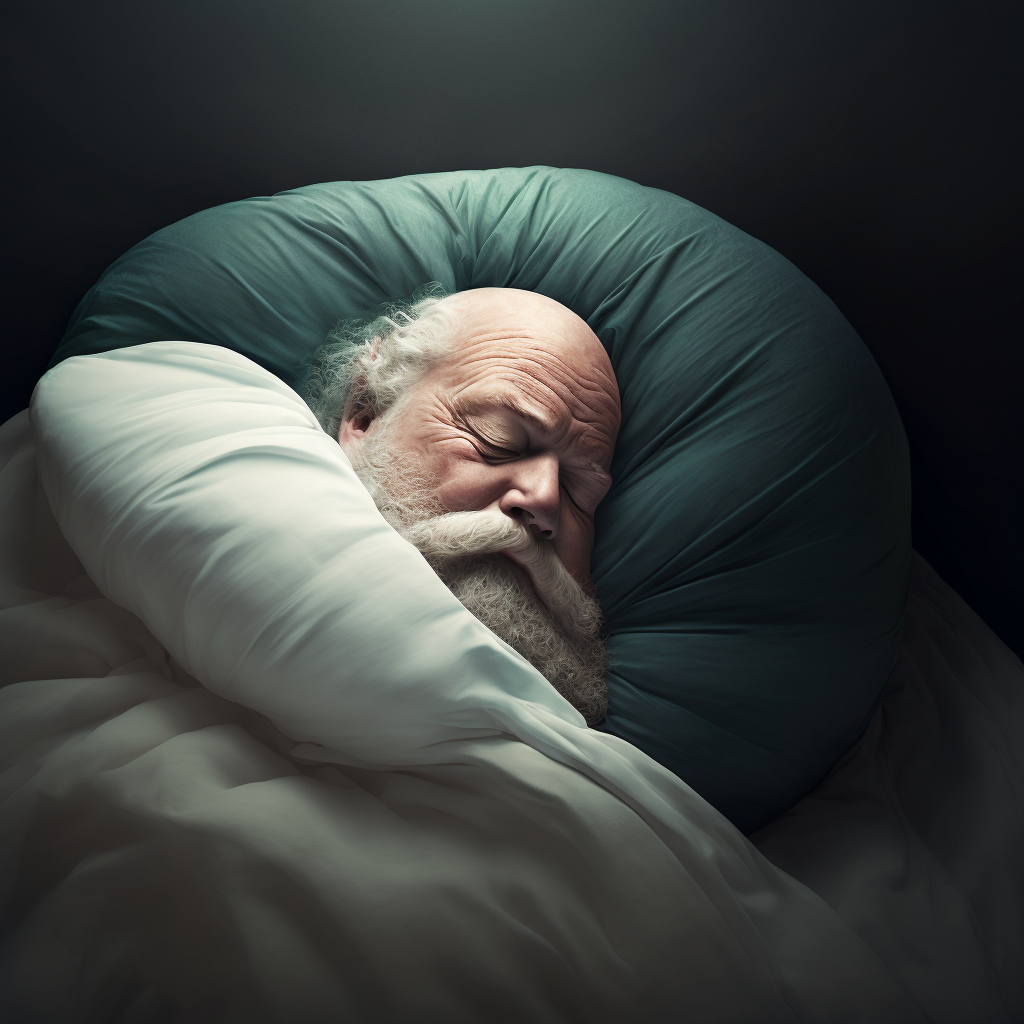
\includegraphics[width=0.48\linewidth]{images/sleep_1.png} \hfill
  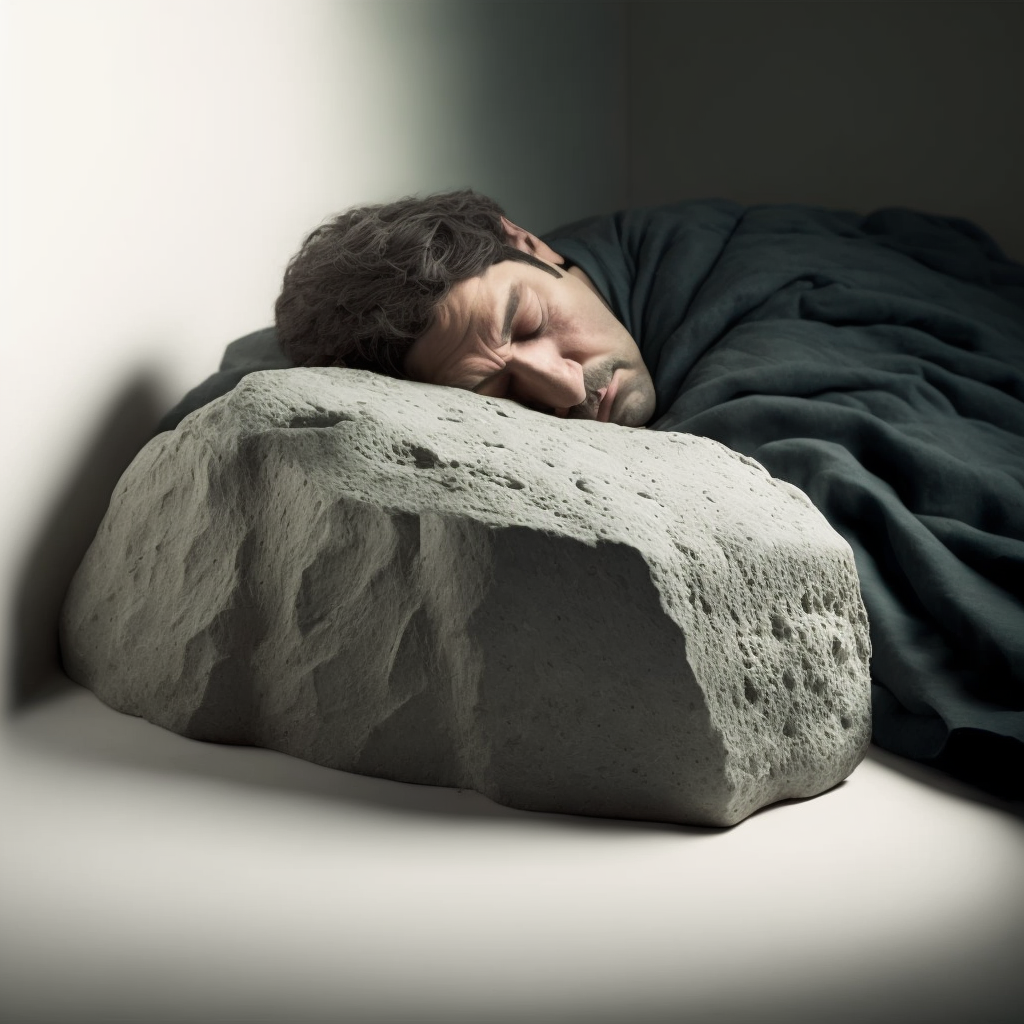
\includegraphics[width=0.48\linewidth]{images/sleep_0.png}
  \caption {Examples of \textit{real} and \textit{weird} images.}
  \label{fig:data}
\end{figure*}

\subsection{Models}

We tested four models for obtaining atomic facts from the images: 
LLaVa \cite{liu2023llava}, BLIP \cite{blip}, GPT-2 \cite{gpt2}, GPT-4o \cite{OpenAI_GPT4_2023}.

For solving the natural language inference task we chose sileod \cite{sileod22-tasknet}, MoritzLaurer \cite{laurer_less_2022} and t5-true \cite{honovich-etal-2022-true-evaluating}.

\subsection{Results}

The comparison results of applying various models from the previous section are presented in Table \ref{tab:acc}.

Reality scores for the whole dataset obtained using \textit{LLaVa} model for captioning and \textit{sileod} model for contradiction detection are presented in Figure \ref{fig:experiments}. Kolmogorov–Smirnov test shows that the distributions are different with one-sided alternative with p-value 4e-5.

\begin{figure}[ht]
  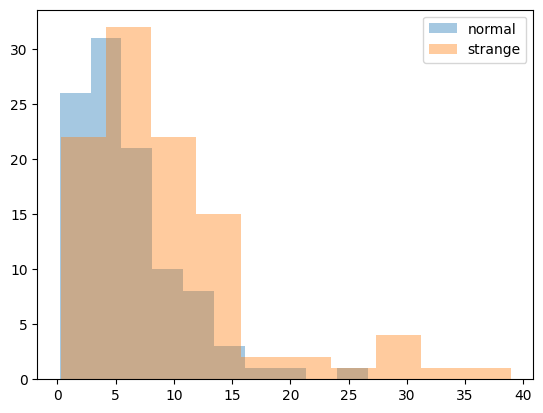
\includegraphics[width=\columnwidth]{images/output.png}
  \caption{Scores distribution.}
  \label{fig:experiments}
\end{figure}

\begin{table}[ht]
    \centering
    \begin{tabular}{c|c c c }
        % \hline
         & sileod & MoritzLaurer & t5-true \\
         \hline
         LLaVa & \textbf{0.68} & 0.42 & 0.63 \\
         BLIP & 0.53 &\textbf{ 0.68} & 0.53 \\
         GPT-2 & 0.37 & 0.32 & 0.37 \\
         GPT-4o & 0.63 & \textbf{0.68} & 0.37 \\
         % \hline
    \end{tabular}
    \caption{Accuracy of various methods.}
    \label{tab:acc}
\end{table}


\section{Conclusion}

In conclusion, the proposed metric for quantifying image realism effectively differentiates between real and weird images by assessing their contextual and commonsense coherence. This approach not only advances the detection of image manipulations and deep-fakes but also enhances AI's ability to align with human perception, ensuring more reliable and nuanced evaluations of visual content. By focusing on how believable the scenarios in images are, we create smarter AI systems that can better understand and interpret the real world.

% Bibliography entries for the entire Anthology, followed by custom entries
%\bibliography{anthology,custom}
% Custom bibliography entries only
\bibliography{custom}

% \appendix

% \section{Example Appendix}
% \label{sec:appendix}

% This is an appendix.

\end{document}
